\documentclass[11pt]{article}

% Load package
\usepackage{../lesson}
\setcounter{MaxMatrixCols}{20}

% Set title and course name
\settitle{Problem Set 2}
\setsubtitle{Markov Processes and Markov Decision Processes}
\setcourse{CME241 - Reinforcement Learning for Finance}
\setdate{Due: 23.01.2023}

\begin{document}

% Create title and add proper header for first page
\maketitle
\thispagestyle{first}

\section{Snakes and Ladders}
\subsection{State Space}
The state space of the snakes and ladders game is simple, it is defined as the square that the player currently occupies.
$$S_t \in \mathcal{S} = \{0,..., 100\}$$

\subsection{Transition Probabilities}
The transition probabilities can be defined by a Categorical distribution over the six numbers consequtively larger than the current state space. However, we must also take account of the snakes and ladders so defining the mapping of state landed on to state ending at as:
\begin{verbatim}
    Mapping[State_landed]->State_ended
\end{verbatim}
We have:
$$
\mathbb{P}[S_{t+1}|S_t] = \text{Categorical(Mapping[$S_{t}+i$]: $\frac{1}{6}$) } \forall i \in [1, 6]
$$

\subsection{Sample Trace and Step Count Plots}
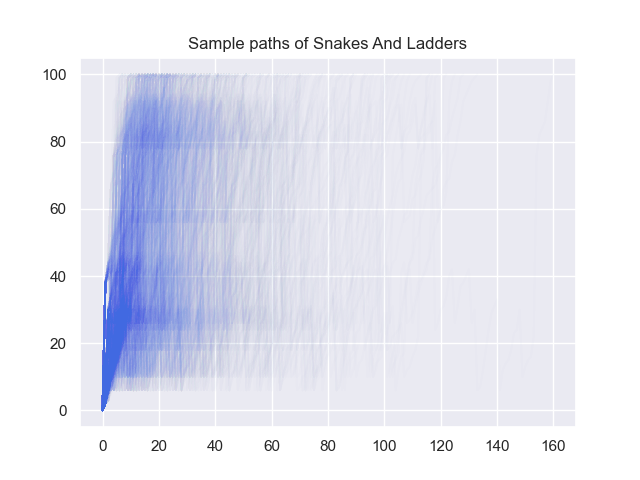
\includegraphics[width=0.49\linewidth]{Q1. Sample paths of Snakes and Ladders.png}
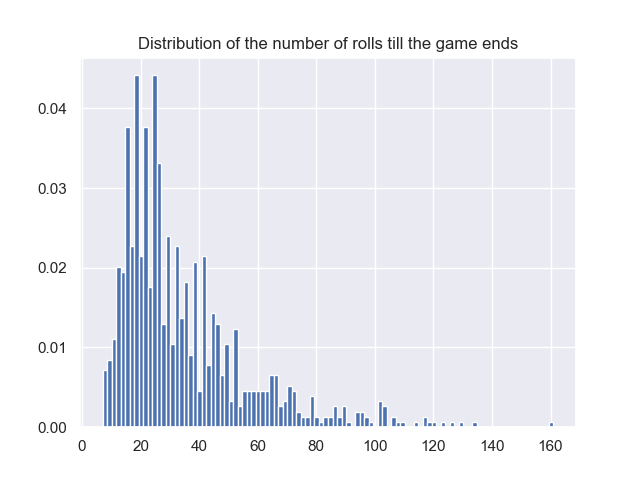
\includegraphics[width=0.49\linewidth]{Q1. Distribution of time to finish.png}

\subsection{Expected Number of Rolls}
By making the snakes and ladder game a Markov Reward Process with a unit reward for every step taken the value function of the reward process will determine the expected number of dice rolls to finish the game. Implementing this for our game given an expected number of rolls as $34.369$ or $35$.

\newpage
\section{Frog Jumps}
\subsection{State Space}
The state space of the frog jump is simple, it is defined as the lilypad that the frog currently occupies.
$$S_t \in \mathcal{S} = \{S, 1, 2, 3, ..., 9, E\}$$
The transition probabilities can thus be written as:
$$
\begin{Bmatrix}
    & 1 & 2 & 3 & 4 & 5 & 6 & 7 & 8 & 9 & E\\
   S & \frac{1}{10} & \frac{1}{10} & \frac{1}{10} & \frac{1}{10} & \frac{1}{10} & \frac{1}{10} & \frac{1}{10} & \frac{1}{10} & \frac{1}{10}& \frac{1}{10}\\
   1 & 0 & \frac{1}{9} & \frac{1}{9} & \frac{1}{9} & \frac{1}{9} & \frac{1}{9} & \frac{1}{9} & \frac{1}{9} & \frac{1}{9}& \frac{1}{9}\\
   2 & 0 & 0 & \frac{1}{8} & \frac{1}{8} & \frac{1}{8} & \frac{1}{8} & \frac{1}{8} & \frac{1}{8} & \frac{1}{8}& \frac{1}{8}\\
   3 & 0 & 0 & 0 & \frac{1}{7} & \frac{1}{7} & \frac{1}{7} & \frac{1}{7} & \frac{1}{7} & \frac{1}{7}& \frac{1}{7}\\
   4 & 0 & 0 & 0 & 0 & \frac{1}{6} & \frac{1}{6} & \frac{1}{6} & \frac{1}{6} & \frac{1}{6}& \frac{1}{6}\\
   5 & 0 & 0 & 0 & 0 & 0 & \frac{1}{5} & \frac{1}{5} & \frac{1}{5} & \frac{1}{5}& \frac{1}{5}\\
   6 & 0 & 0 & 0 & 0 & 0 & 0 & \frac{1}{4} & \frac{1}{4} & \frac{1}{4} & \frac{1}{4}\\
   7 & 0 & 0 & 0 & 0 & 0 & 0 & 0 & \frac{1}{3} & \frac{1}{3}& \frac{1}{3}\\
   8 & 0 & 0 & 0 & 0 & 0 & 0 & 0 & 0 & \frac{1}{2}& \frac{1}{2}\\
   9 & 0 & 0 & 0 &0 & 0 & 0 & 0 & 0 & 0 & 1
\end{Bmatrix}
$$

\subsection{Expected Number of Jumps}
The expected number of jumps for this process is $2.93$. This can be calculated by solving the states value functions regressively from the end state (setting the Reward identically to 1):
\begin{align}
    V(E) &= 0\\
    V(9) &= 1 + \sum_{s'\in\mathcal{N}} \frac{1}{1} V(s') = 1\\
    V(8) &= 1 + \sum_{s'\in\mathcal{N}} \frac{1}{2} V(s') = 1.5\\
    V(7) &= 1 + \sum_{s'\in\mathcal{N}} \frac{1}{3} V(s') = \frac{11}{6}\\
    V(6) &= 1 + \sum_{s'\in\mathcal{N}} \frac{1}{4} V(s') = \frac{25}{12}\\
    V(5) &= 1 + \sum_{s'\in\mathcal{N}} \frac{1}{5} V(s') = \frac{137}{60}\\
    V(4) &= 1 + \sum_{s'\in\mathcal{N}} \frac{1}{6} V(s') = \frac{49}{20}\\
    V(3) &= 1 + \sum_{s'\in\mathcal{N}} \frac{1}{7} V(s') = \frac{363}{140}\\
    V(2) &= 1 + \sum_{s'\in\mathcal{N}} \frac{1}{8} V(s') = \frac{761}{280}\\
    V(1) &= 1 + \sum_{s'\in\mathcal{N}} \frac{1}{9} V(s') = \frac{7129}{2520}\\
    V(S) &= 1 + \sum_{s'\in\mathcal{N}} \frac{1}{10} V(s') = \frac{7381}{2520} = 2.93
\end{align}

\subsection{Closed Form for Expected Jumps}
When solving the above form we find the closed form solution mirrors a harmonic sequence:
\begin{align}
    V(9) &= 1 \\
    V(8) &= 1 + \frac{1}{2} \\
    V(7) &= 1 + \frac{1}{2} + \frac{1}{3} \\
    V(6) &= ... \\
    V(0) &= \sum_{i=1}^n \frac{1}{n}
\end{align}

\newpage
\section{MDP}
\subsection{Optimal Value Function}
The optimal value function for a MDP is defined as:
$$
V^*(s) = \max_{a\in\mathcal{A}} \left\{\mathcal{R}(s, a) + \gamma\sum_{s'\in\mathcal{N}}\mathcal{P}(s, a, s')\cdot V^*(s') \right\}
$$

In our case we have the reward from a state determined by the probability $a$, i.e. 
\begin{align}
    \mathcal{R}(s, a) &= \sum_{a\in\mathcal{A}}r_a\cdot\P{a|s = s} \\
                      &= a(1 - a) + (1-a)(1+a) \\
                      &= 1 + a - 2a^2 \\
\end{align}

We can also simplify the second term to:
\begin{align}
    \gamma\sum_{s'\in\mathcal{N}}\mathcal{P}(s, a, s')\cdot V^*(s') = \gamma(aV^*(s) + (1-a)V^*(s-1)) \\
\end{align}
Since we have an infinite process we also know that $V^*(s) = V^*(s+1)$, giving:
\begin{align}
    &= \gamma aV^*(s) + \gamma(1-a)V^*(s) \\
    &= \gamma V^*(s)
\end{align}
Combining this gives us the value function as:
\begin{align}
    V^*(s) = \max_{a\in\mathcal{A}} \left\{1 + a - 2a^2 + \gamma V^*(s) \right\}\\
    V^*(s)(1 - \gamma) &= 1 + a  - 2a^2 \\
    V^*(s) = &= 2 * (1 + a - 2a^2)
\end{align}
Optimising this with respect to $a$, we take the partial derivative w.r.t. $a$:
$$
\frac{\partial}{\partial a} 2 + 2a - 4a^2 = 2 - 8a = 0
$$
Solving this gives:
$$
a = \frac{1}{4}; V^*(s) = \frac{9}{4}
$$

\end{document}